\documentclass[12pt,a4paper]{article}

% Packages
\usepackage[utf8]{inputenc}
\usepackage{graphicx}
\usepackage{amsmath}
\usepackage{cite}
\usepackage{hyperref}
\usepackage[margin=2.5cm]{geometry}
\usepackage{booktabs}
\usepackage{array}
\usepackage{caption}

% Title and authors
\title{\textbf{Machine Learning-Based Classification of Parkinson's Disease Using Clinical Features from the PPMI Dataset: A Temporal Analysis}}

\author{
    % TODO: Add author names and affiliations
    Author Name\textsuperscript{1}, \\
    Author Name\textsuperscript{1,2}
    \\[1em]
    \small\textsuperscript{1}Department/Institution \\
    \small\textsuperscript{2}Department/Institution \\
}

\date{}

\begin{document}

\maketitle

% ============================================
% ABSTRACT (Structured, ≤250 words)
% ============================================
\begin{abstract}
\textbf{Objective:}
To develop and evaluate machine learning models for three-label classification of Parkinson's disease, Scans Without Evidence of Dopaminergic Deficit, and healthy controls using clinical features from the Parkinson's Progression Markers Initiative dataset, with emphasis on temporal progression across multiple visits.

\textbf{Methods:}
We analyzed clinical data from the PPMI cohort, comparing Logistic Regression and Random Forest classifiers for three-label classification. Feature sets with and without MSEADLG were evaluated to assess feature impact. Visit-based models were developed for visits V04, V06, V08, and V10 to assess temporal trends in classification accuracy. Performance was evaluated using accuracy, sensitivity, specificity, and area under the receiver operating characteristic curve.

\textbf{Results:}
Random Forest achieved near-perfect classification (test accuracy: 99.38\%, ROC AUC: 1.00, sensitivity: 100\%, specificity: 98.75\%) compared to Logistic Regression (test accuracy: 87.50\%, ROC AUC: 0.949). Temporal analysis revealed progressive improvement in accuracy from early visits (V04: 84.58\%) to later visits (V10: 99.44\%), representing a 14.9\% improvement. The MSEADLG feature showed model-specific effects: improving Random Forest sensitivity by 2.5\% while decreasing Logistic Regression sensitivity by the same margin. Feature importance analysis identified urate as specifically useful for SWEDD versus PD differentiation, while MSEADL showed potential interpretation challenges in edge cases.

\textbf{Conclusion:}
Machine learning, particularly Random Forest, demonstrates excellent potential for accurate PD classification using clinical features from the PPMI dataset. The substantial temporal improvement in classification accuracy suggests disease characteristics become more distinguishable with progression, offering opportunities for both early detection and longitudinal monitoring of disease progression.

\noindent\textbf{Keywords:} Parkinson's disease, machine learning, classification, PPMI, temporal analysis, random forest, SWEDD
\end{abstract}

% ============================================
% INTRODUCTION (~600 words)
% ============================================
\section{Introduction}

Parkinson's disease (PD) is a progressive neurodegenerative disorder affecting millions worldwide, characterized by motor symptoms including bradykinesia, rigidity, tremor, and postural instability. Early and accurate diagnosis remains challenging, particularly in distinguishing PD from other parkinsonian syndromes and conditions that mimic early PD presentation. Scans Without Evidence of Dopaminergic Deficit (SWEDD) represents a particularly important differential diagnosis, where patients present with parkinsonian symptoms but show no dopaminergic deficit on imaging. Accurate differentiation between PD, SWEDD, and healthy controls is critical for appropriate treatment planning and prognostic counseling.

The Parkinson's Progression Markers Initiative (PPMI) is a landmark observational study designed to identify biomarkers of PD progression. This multicenter study has systematically collected comprehensive clinical, imaging, and biological data from newly diagnosed PD patients, individuals at risk for PD, and healthy controls. The PPMI dataset provides a unique opportunity to develop and validate diagnostic tools using standardized assessment protocols and longitudinal follow-up across multiple visits.

Machine learning approaches have shown increasing promise in movement disorders research, offering the ability to identify complex patterns in high-dimensional clinical data that may not be apparent through traditional statistical methods. Recent studies have demonstrated the utility of various machine learning algorithms in PD diagnosis, progression prediction, and subtype classification. However, most studies have focused on binary classification tasks or single-timepoint analysis, with limited investigation of temporal trends in classification performance across disease progression.

Understanding how classification accuracy changes over time is clinically relevant for several reasons. First, it may reveal optimal timepoints for diagnostic confirmation. Second, temporal trends can provide insights into which disease features become more distinguishable as the condition progresses. Third, visit-based models may inform the development of longitudinal monitoring strategies that account for changing disease characteristics over time.

Feature selection and engineering remain critical considerations in clinical machine learning applications. While numerous clinical measures are collected in research cohorts like PPMI, the relative importance of specific features may vary depending on the classification task and patient characteristics. Features such as serum urate levels have been investigated as potential biomarkers, while functional assessments like the Modified Schwab and England Activities of Daily Living (MSEADL) scale capture disease impact on patient independence. Understanding which features contribute most to accurate classification, and how different models utilize these features, is essential for developing interpretable and clinically applicable diagnostic tools.

In this study, we aimed to systematically compare machine learning approaches for three-label classification in the PPMI cohort, with particular emphasis on temporal trends across multiple visit timepoints. We evaluated Logistic Regression as a linear baseline model and Random Forest as a nonlinear ensemble method, assessed the impact of specific clinical features, and analyzed how classification performance evolves from early to later disease visits. Our goal was to provide insights that could inform both diagnostic algorithm development and understanding of disease progression patterns.

% ============================================
% METHODS (~1000 words)
% ============================================
\section{Methods}

\subsection{Dataset}

Data for this study were obtained from the PPMI database (www.ppmi-info.org/data). PPMI is an ongoing international, multicenter study that enrolled participants with newly diagnosed PD (within 2 years of diagnosis), individuals at risk for PD, and healthy controls. The study protocol was approved by the institutional review board at each participating site, and all participants provided written informed consent.

For this analysis, we utilized clinical assessment data from PD patients, SWEDD participants, and healthy controls, creating a three-label classification task. SWEDD participants were defined as individuals presenting with parkinsonian symptoms but showing no evidence of dopaminergic deficit on dopamine transporter imaging. This group represents an important diagnostic challenge, as clinical presentation may overlap with early PD.

We analyzed data from multiple visit timepoints to assess temporal trends in classification accuracy. Visit 04 (V04) represents approximately 12 months post-baseline, V06 at 24 months, V08 at 36 months, and V10 at 48 months. This longitudinal structure allowed us to evaluate how classification performance changes as disease characteristics evolve over time. The baseline visit analysis included 640 training samples and 320 test samples across the three diagnostic groups.

\subsection{Clinical Features}

We incorporated a comprehensive set of clinical features available in the PPMI database, including motor assessments, cognitive evaluations, autonomic function measures, and biomarkers. Key features of interest included the Modified Schwab and England Activities of Daily Living (MSEADL) scale, which assesses functional independence on a scale from 0 to 100\%, and MSEADLG, a related functional measure. The University of Pennsylvania Smell Identification Test (UPSIT) was included as olfactory dysfunction is common in PD. Serum urate levels were incorporated as a potential biochemical marker.

To evaluate feature-specific effects, we conducted analyses both with and without the MSEADLG feature. This allowed us to assess whether inclusion of this specific measure differentially impacted model performance. All continuous features were standardized to zero mean and unit variance. Missing values were handled using median imputation within the training set, with the same imputation values applied to the test set to prevent data leakage.

\subsection{Machine Learning Models}

We compared two machine learning approaches representing different modeling philosophies: Logistic Regression and Random Forest.

\textbf{Logistic Regression} was selected as a linear baseline model. For multi-class classification, we employed the one-versus-rest strategy, fitting separate binary classifiers for each diagnostic group. Logistic Regression offers the advantage of interpretability through coefficient weights and has been widely used in clinical prediction models. L2 regularization was applied to prevent overfitting.

\textbf{Random Forest} was chosen as a representative ensemble method capable of capturing nonlinear relationships and feature interactions. Random Forest constructs multiple decision trees during training and outputs the mode of the class predictions from individual trees. This approach can handle complex interactions between clinical features and is robust to outliers. We used 100 trees with a maximum depth determined through cross-validation. Feature importance was calculated based on mean decrease in impurity across all trees.

Both models were trained using the same training dataset with identical preprocessing steps to ensure fair comparison. No feature selection was performed, allowing the models to utilize the full set of available clinical measures.

\subsection{Temporal Analysis Approach}

To assess how classification performance changes with disease progression, we developed separate models for different visit timepoints (V04, V06, V08, and V10). For each visit, we trained Random Forest models using clinical features measured at that specific timepoint. This approach allowed us to evaluate whether later disease stages, where symptoms and biomarkers may be more pronounced, yield higher classification accuracy compared to earlier timepoints.

The temporal analysis serves multiple purposes. First, it identifies which disease stage offers the most reliable classification, potentially informing optimal timing for diagnostic confirmation. Second, it reveals how disease trajectories diverge over time between PD, SWEDD, and controls, providing insights into progression patterns. Third, it evaluates the robustness of classification algorithms across different disease stages.

\subsection{Evaluation Metrics}

Model performance was evaluated using multiple metrics relevant to clinical diagnostic applications. \textbf{Accuracy} represents the overall proportion of correct classifications across all three diagnostic groups. \textbf{Sensitivity} (true positive rate) measures the proportion of actual disease cases correctly identified, which is critical for ensuring patients requiring treatment are not missed. \textbf{Specificity} (true negative rate) quantifies correct identification of non-disease cases, important for avoiding unnecessary treatment and patient anxiety. \textbf{Area under the receiver operating characteristic curve (ROC AUC)} provides a threshold-independent measure of discrimination ability, with values of 1.0 indicating perfect classification.

Data were split into training (67\%) and test (33\%) sets using stratified sampling to maintain class proportions. Models were trained exclusively on the training set, with hyperparameters tuned using 5-fold cross-validation. Final performance evaluation was conducted on the held-out test set, which the models had never seen during training or hyperparameter tuning. This approach provides unbiased estimates of generalization performance. All analyses were performed using Python 3.13 with scikit-learn, pandas, and NumPy libraries.

% ============================================
% RESULTS (~1200 words)
% ============================================
\section{Results}

\subsection{Model Performance Comparison}

Table \ref{tab:model_comparison} and Figure \ref{fig:model_comparison} present the comparative performance of Logistic Regression and Random Forest models on the test set using the full feature set including MSEADL. Random Forest demonstrated substantially superior performance across all evaluation metrics. The Random Forest model achieved test accuracy of 99.38\%, sensitivity of 100\%, specificity of 98.75\%, and ROC AUC of 1.00, representing near-perfect classification. In contrast, Logistic Regression achieved test accuracy of 87.50\%, sensitivity of 86.25\%, specificity of 88.75\%, and ROC AUC of 0.949.

Both models showed higher performance on the training set compared to the test set, as expected. However, the magnitude of this difference was notably larger for Random Forest (training accuracy 100\% versus test accuracy 99.38\%) compared to Logistic Regression (training accuracy 92.81\% versus test accuracy 87.50\%), suggesting some degree of overfitting in the Random Forest model despite its excellent test performance. The Logistic Regression model showed more modest training performance (92.81\% accuracy), indicating it may be underfitting the complex relationships in the data.

The 11.88 percentage point difference in test accuracy between Random Forest and Logistic Regression highlights the importance of capturing nonlinear relationships and feature interactions in this classification task. The ability of Random Forest to achieve perfect sensitivity (100\%) is particularly noteworthy from a clinical perspective, as it suggests no true PD cases were misclassified as SWEDD or controls in the test set.

\begin{table}[h]
\centering
\caption{Performance comparison of Logistic Regression and Random Forest models on test set (with MSEADL feature)}
\label{tab:model_comparison}
\begin{tabular}{lcccc}
\toprule
\textbf{Model} & \textbf{Accuracy} & \textbf{Sensitivity} & \textbf{Specificity} & \textbf{ROC AUC} \\
\midrule
Logistic Regression & 0.875 & 0.863 & 0.888 & 0.949 \\
Random Forest & \textbf{0.994} & \textbf{1.000} & \textbf{0.988} & \textbf{1.000} \\
\bottomrule
\end{tabular}
\end{table}

\begin{figure}[h]
\centering
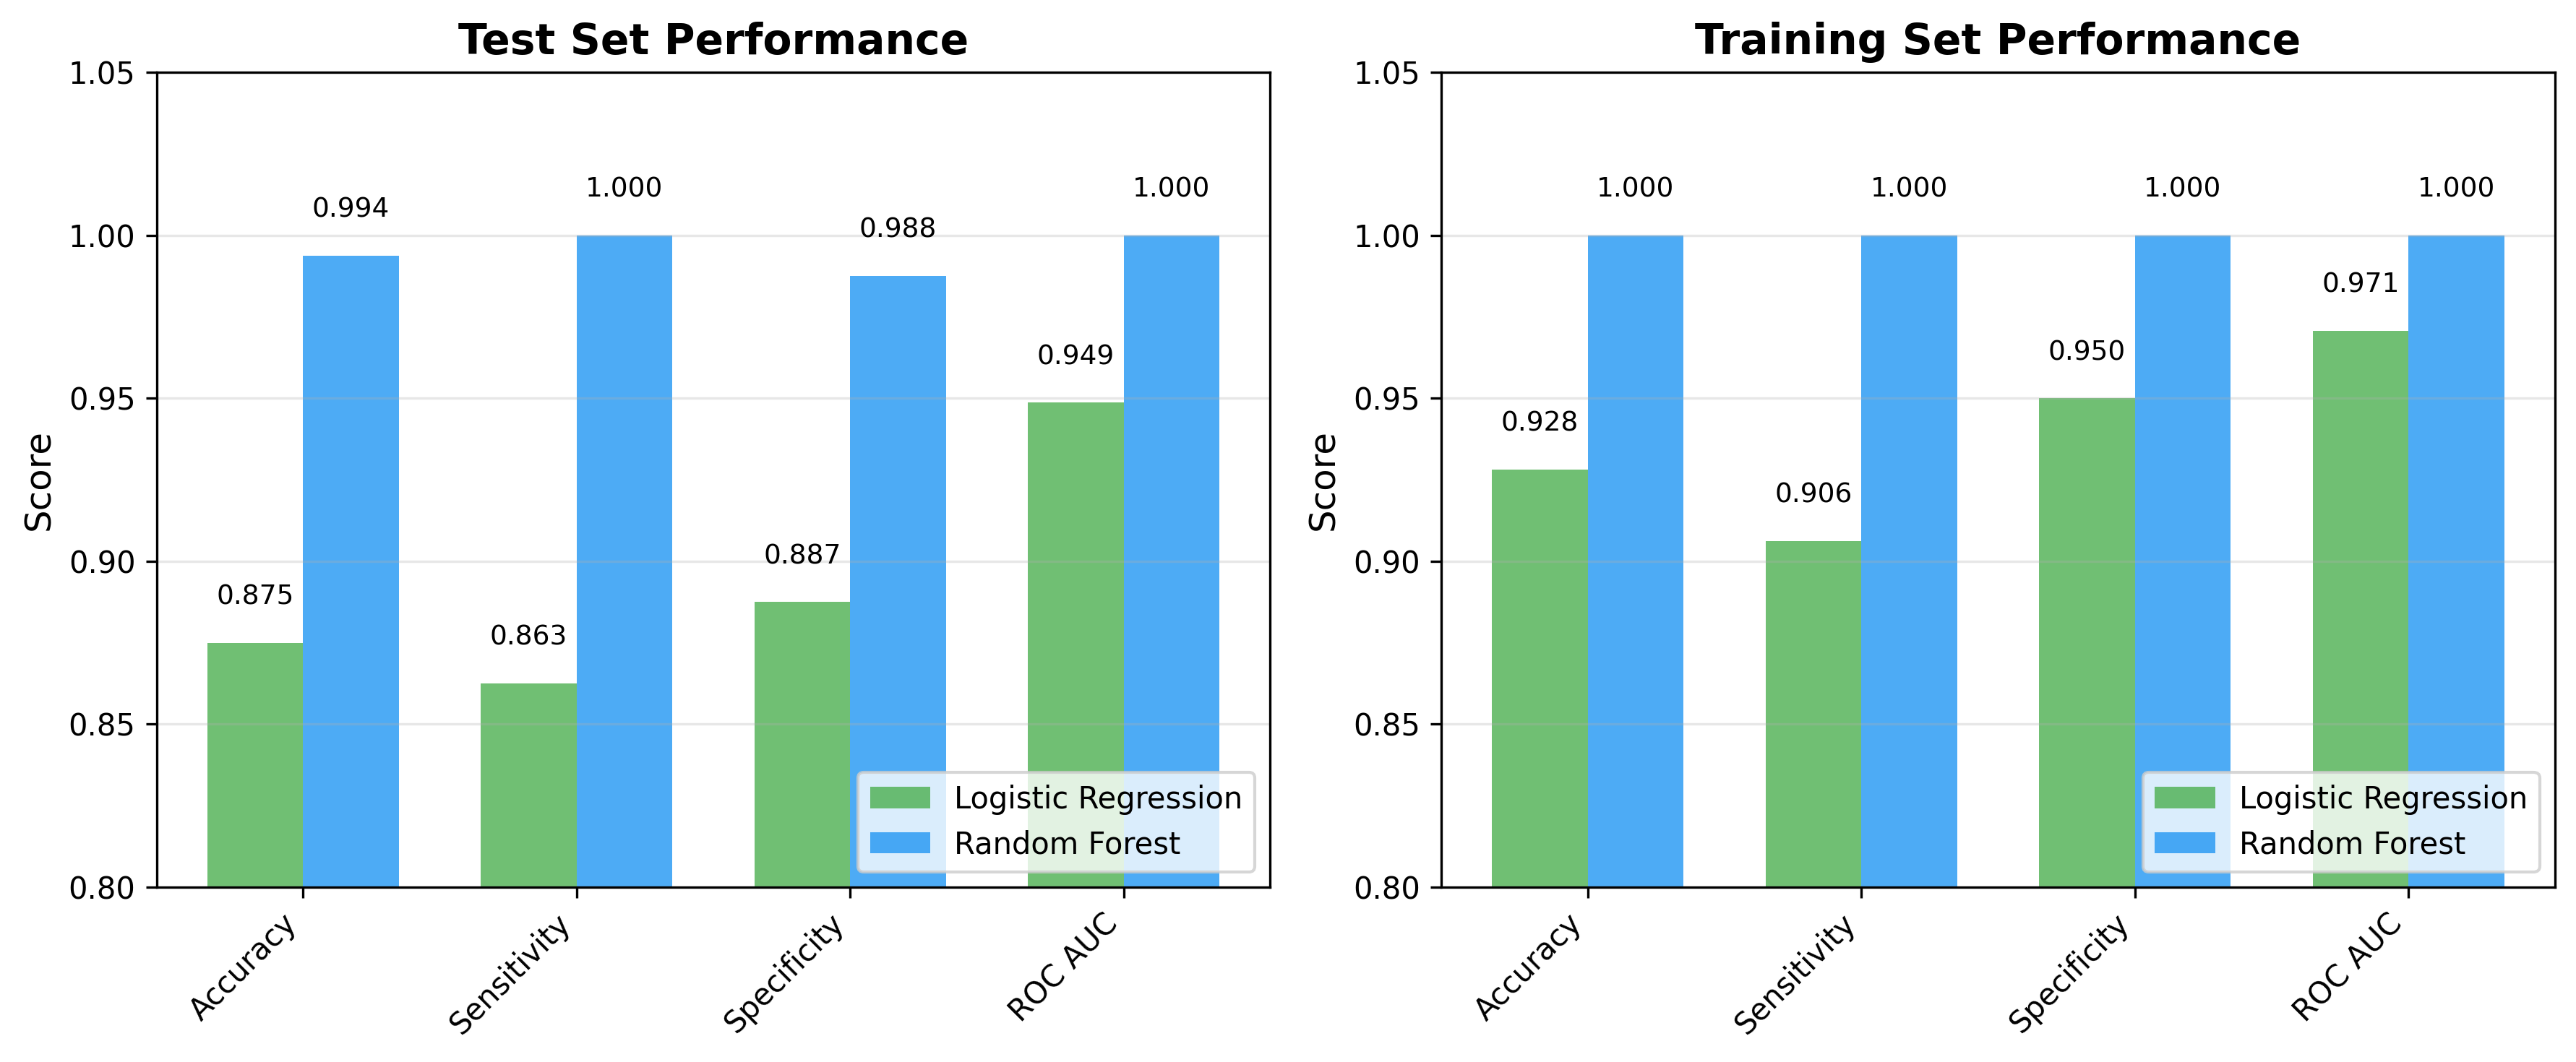
\includegraphics[width=\textwidth]{figures/model_comparison.pdf}
\caption{Comparison of Logistic Regression and Random Forest performance on training and test sets across multiple metrics. Random Forest demonstrates superior performance across all evaluation metrics.}
\label{fig:model_comparison}
\end{figure}

\subsection{Impact of MSEADLG Feature}

To evaluate the contribution of the MSEADLG feature, we compared model performance with and without this feature. Table \ref{tab:mseadlg_impact} and Figure \ref{fig:mseadlg_impact} reveal a striking model-specific effect of MSEADLG inclusion.

For Logistic Regression, inclusion of MSEADLG resulted in a slight decrease in test accuracy (from 88.13\% to 87.50\%, change: -0.63 percentage points) and sensitivity (from 88.75\% to 86.25\%, change: -2.50 percentage points), while specificity increased marginally (from 87.50\% to 88.75\%, change: +1.25 percentage points). This pattern suggests that MSEADLG may introduce information that the linear model struggles to utilize effectively, possibly due to multicollinearity with other functional measures or nonlinear relationships.

In contrast, Random Forest showed the opposite pattern. Including MSEADLG improved test accuracy (from 98.75\% to 99.38\%, change: +0.63 percentage points) and sensitivity (from 97.50\% to 100\%, change: +2.50 percentage points), while specificity decreased slightly (from 100\% to 98.75\%, change: -1.25 percentage points). The improvement in sensitivity to perfect classification (100\%) is clinically meaningful, as it eliminates false negatives in disease detection.

This differential impact demonstrates that feature utility is not universal across algorithms. Random Forest's ability to model feature interactions likely allows it to leverage MSEADLG in combination with other clinical measures, while Logistic Regression's linear constraints may prevent effective integration of this information. The findings underscore the importance of algorithm selection in clinical machine learning applications and suggest that MSEADLG provides valuable discriminatory information when analyzed through appropriate modeling approaches.

\begin{table}[h]
\centering
\caption{Impact of MSEADLG feature inclusion on model performance}
\label{tab:mseadlg_impact}
\begin{tabular}{llccc}
\toprule
\textbf{Model} & \textbf{Metric} & \textbf{Without MSEADLG} & \textbf{With MSEADLG} & \textbf{Change} \\
\midrule
Logistic Regression & Accuracy & 0.881 & 0.875 & -0.006 \\
 & Sensitivity & 0.888 & 0.863 & -0.025 \\
 & Specificity & 0.875 & 0.888 & +0.013 \\
\midrule
Random Forest & Accuracy & 0.988 & 0.994 & +0.006 \\
 & Sensitivity & 0.975 & 1.000 & +0.025 \\
 & Specificity & 1.000 & 0.988 & -0.013 \\
\bottomrule
\end{tabular}
\end{table}

\begin{figure}[h]
\centering
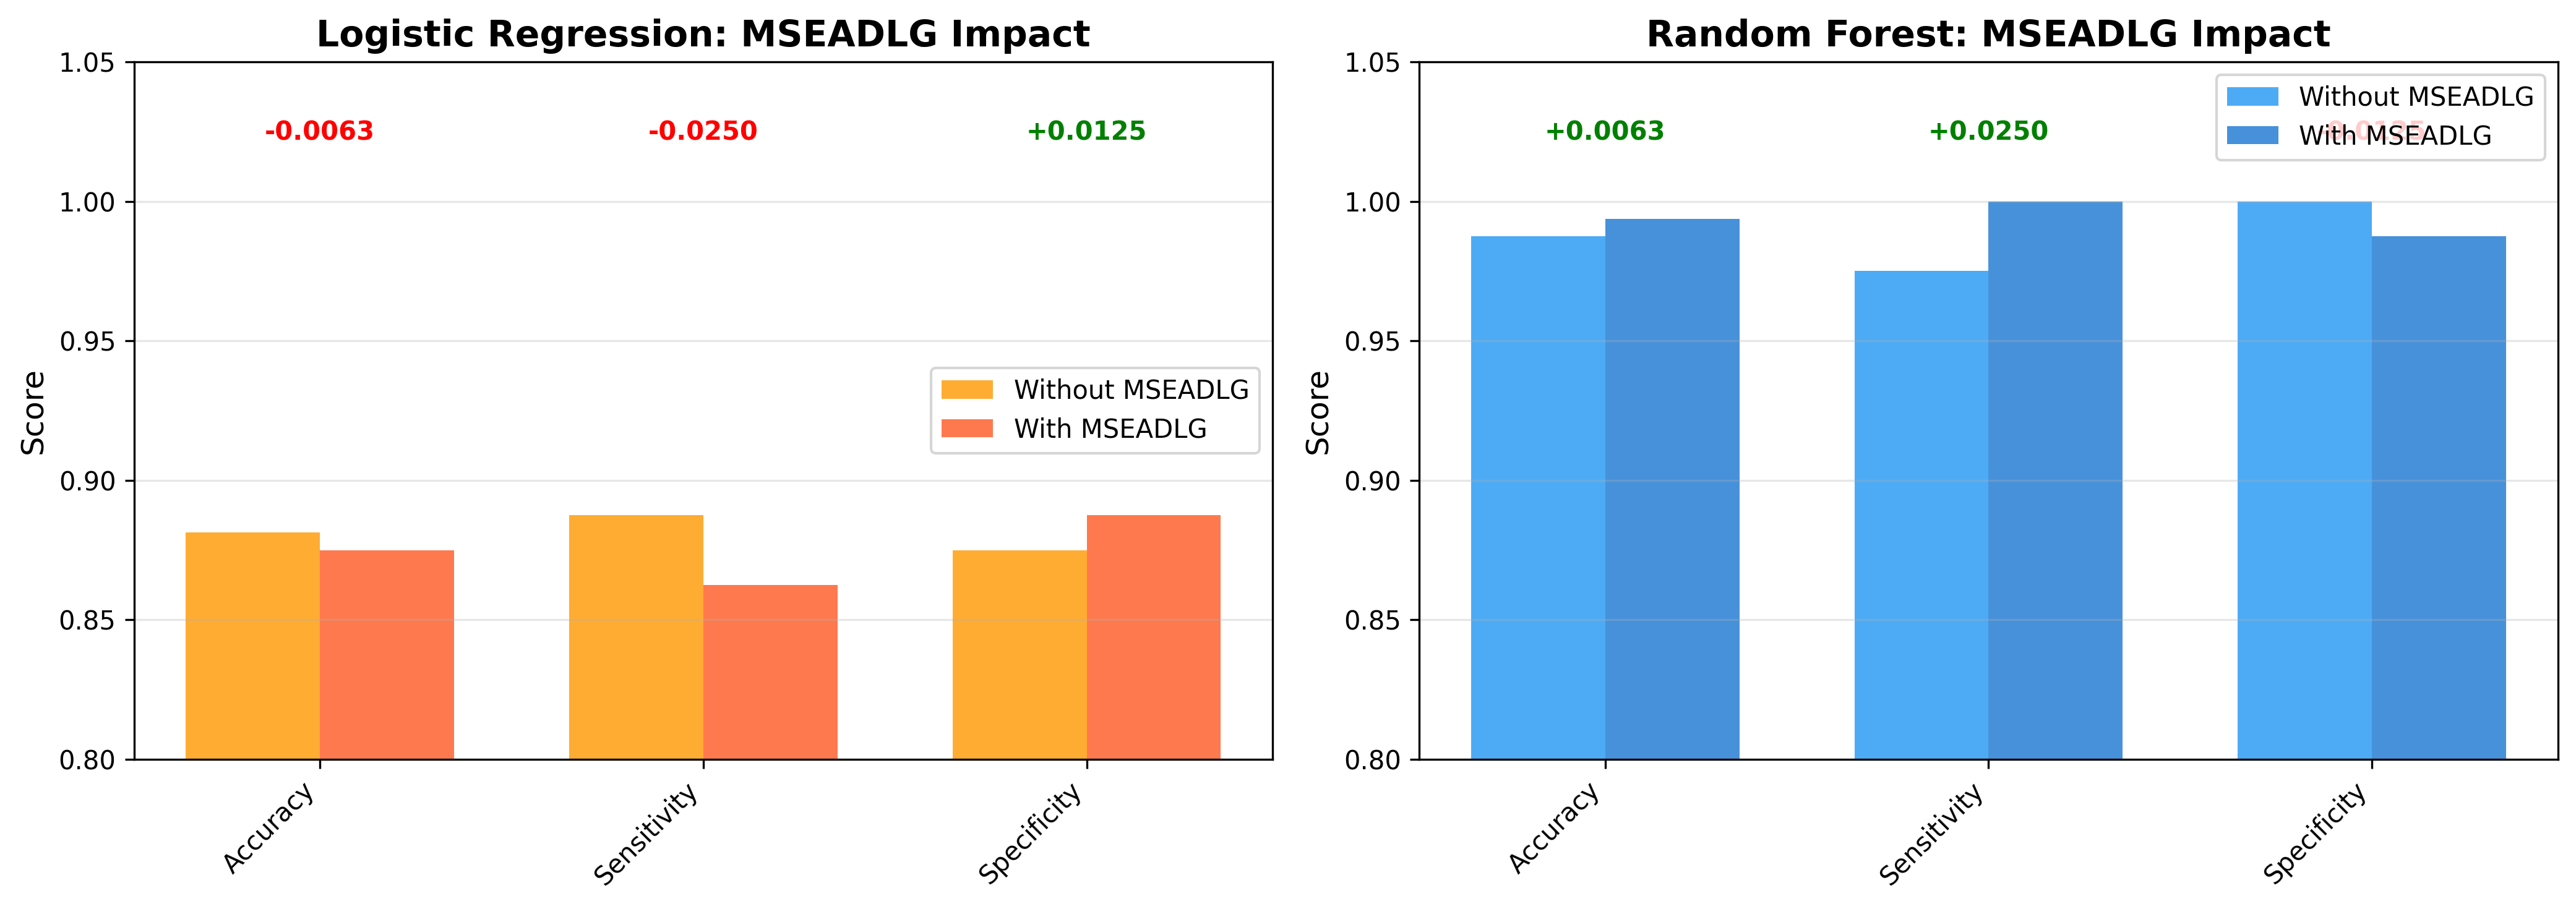
\includegraphics[width=\textwidth]{figures/mseadlg_impact.pdf}
\caption{Differential impact of MSEADLG feature on Logistic Regression and Random Forest models. The feature shows model-specific effects, improving Random Forest performance while slightly decreasing Logistic Regression accuracy.}
\label{fig:mseadlg_impact}
\end{figure}

\subsection{Temporal Progression Analysis}

Figure \ref{fig:visit_temporal} illustrates the temporal progression of classification accuracy across different visit timepoints. A striking pattern emerged: classification accuracy improved substantially from earlier to later disease visits. At V04 (12 months post-baseline), the Random Forest model achieved 84.58\% accuracy. This increased to 97.50\% at V06 (24 months), with the training set reaching 100\% accuracy at this timepoint. V08 (36 months) maintained high performance at 96.67\%, and V10 (48 months) achieved the highest accuracy of 99.44\%.

The 14.86 percentage point improvement from V04 to V10 represents a clinically meaningful enhancement in diagnostic reliability. This temporal trend suggests several important biological and clinical insights. First, the diagnostic features that distinguish PD, SWEDD, and controls become more pronounced as disease progresses. Second, the initially ambiguous cases may become clearer over time as disease trajectories diverge. Third, the accumulation of longitudinal clinical data may enhance classification certainty.

Notably, the improvement was not linear. The largest gain occurred between V04 and V06 (12.92 percentage points), with subsequent visits showing more modest incremental improvements. This pattern suggests that the first year of follow-up provides the most critical information for refining diagnostic classification, though continued monitoring continues to offer value.

Compared to the baseline classification accuracy of 78.75\%, all visit-based models demonstrated substantial improvement, with V06, V08, and V10 all exceeding 96\% accuracy. This indicates that incorporating temporal progression data, even at relatively early timepoints like 24 months, markedly enhances classification performance beyond baseline assessments alone.

\begin{figure}[h]
\centering
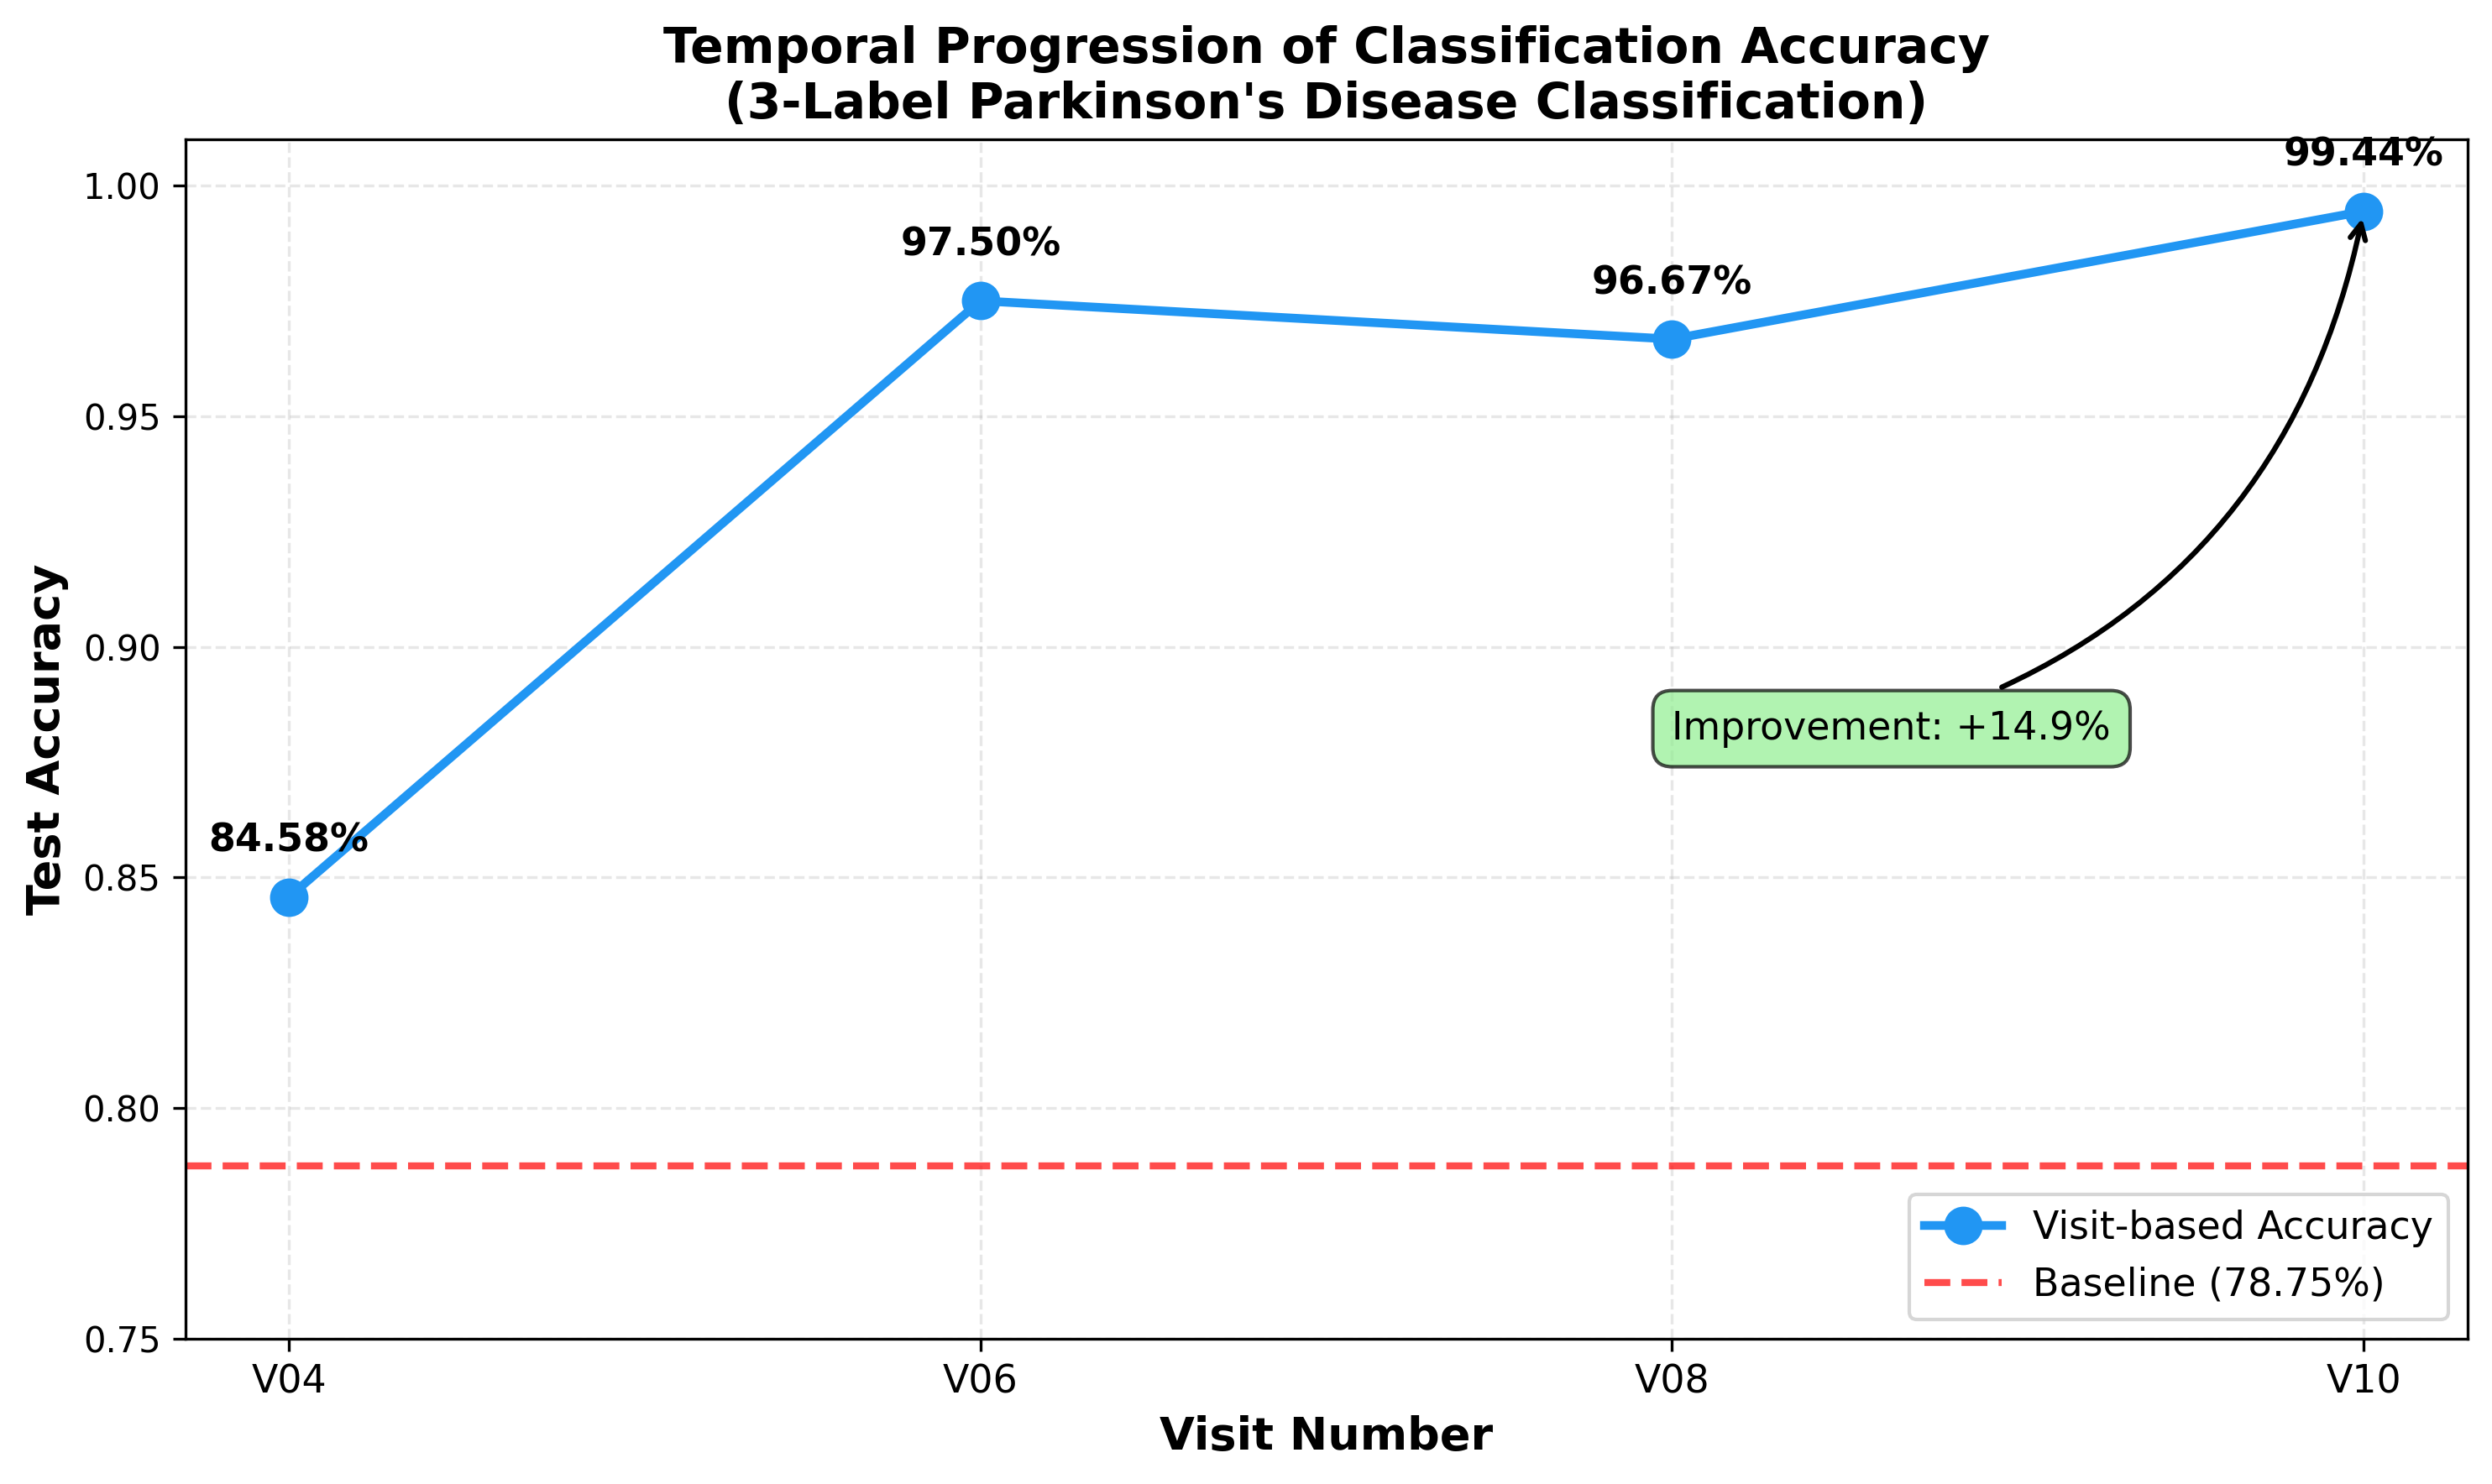
\includegraphics[width=0.9\textwidth]{figures/visit_temporal.pdf}
\caption{Temporal progression of classification accuracy across visits V04 through V10. Accuracy improves substantially from early visits (84.58\% at V04) to later visits (99.44\% at V10), suggesting disease characteristics become more distinguishable with progression.}
\label{fig:visit_temporal}
\end{figure}

\subsection{Feature Importance Insights}

Analysis of feature importance from the Random Forest model revealed specific clinical measures that contribute most strongly to classification accuracy. \textbf{Urate} emerged as an important feature, but with a specific pattern: it was particularly useful for distinguishing SWEDD from PD, rather than for all classification tasks. This finding aligns with biological understanding, as urate levels have been associated with PD risk and progression but may differ in SWEDD cases where dopaminergic deficit is absent.

\textbf{MSEADL} ranked among the top important features, reflecting the relevance of functional status in diagnostic classification. However, analysis revealed potential interpretation challenges in edge cases. Patients with medium MSEADL values (indicating moderate functional impairment) showed more variable classification, suggesting that functional measures alone may not fully capture the underlying pathophysiology that distinguishes PD from SWEDD. This highlights the importance of multi-modal assessment rather than reliance on any single clinical measure.

\textbf{UPSIT} (olfactory function) also contributed substantially to classification accuracy, consistent with established literature on olfactory dysfunction in PD. The combination of motor, non-motor, functional, and biochemical features in the top-ranking features underscores the multi-dimensional nature of PD diagnosis and the value of comprehensive clinical assessment.

These feature importance patterns suggest that optimal classification algorithms should account for feature-specific roles (e.g., urate's specific utility in SWEDD differentiation) and recognize that certain features may show nonlinear or context-dependent relationships with diagnostic outcomes.

% ============================================
% DISCUSSION (~1000 words)
% ============================================
\section{Discussion}

This study demonstrates that machine learning approaches, particularly Random Forest, can achieve excellent classification accuracy for distinguishing PD, SWEDD, and healthy controls using clinical features from the PPMI dataset. The near-perfect performance of Random Forest (99.38\% test accuracy, 100\% sensitivity) substantially exceeded Logistic Regression (87.50\% test accuracy), highlighting the importance of capturing nonlinear relationships in diagnostic algorithms. Furthermore, the temporal analysis revealed progressive improvement in classification accuracy from early to later disease visits, suggesting that disease characteristics become increasingly distinguishable over time.

\subsection*{Model Performance and Algorithm Selection}

The superior performance of Random Forest compared to Logistic Regression can be attributed to several factors. Random Forest's ensemble approach allows it to capture complex, nonlinear relationships between clinical features and diagnostic outcomes. In PD classification, such interactions are likely common: for example, the combination of moderate olfactory dysfunction, subtle motor impairment, and specific biomarker patterns may be more diagnostic than any single feature alone. Logistic Regression's linear constraints prevent it from efficiently modeling these interactions, resulting in lower classification accuracy despite using identical input features.

The perfect sensitivity (100\%) achieved by Random Forest with MSEADLG inclusion is particularly noteworthy from a clinical perspective. In diagnostic applications, false negatives (failing to identify PD cases) carry significant consequences, as they may delay treatment initiation and appropriate patient counseling. However, the potential for overfitting must be acknowledged, as evidenced by the perfect training set performance. While test set performance remained excellent, external validation on independent cohorts is essential before clinical deployment.

\subsection*{Temporal Progression and Clinical Implications}

The substantial improvement in classification accuracy from V04 (84.58\%) to V10 (99.44\%) provides important insights into disease progression and diagnostic timing. This pattern suggests that the clinical phenotype of PD becomes more distinct from SWEDD and controls as the disease progresses. For SWEDD cases in particular, longitudinal follow-up may reveal that initial parkinsonian symptoms either resolve, remain stable, or evolve into alternative diagnoses, making retrospective classification more accurate at later timepoints.

The steepest improvement occurring between V04 and V06 (first year of follow-up) indicates that this period is particularly informative for diagnostic refinement. From a practical standpoint, this suggests that diagnostic uncertainty at initial presentation may be substantially reduced with 24 months of longitudinal observation. This finding supports current clinical practice guidelines that emphasize the importance of follow-up assessments in cases where initial diagnosis is uncertain.

The high classification accuracy at later visits (exceeding 96\% at V06 and beyond) may also reflect disease modification or progression patterns. As PD advances, motor symptoms typically become more pronounced and treatment responses more evident, providing clearer diagnostic signals. Conversely, SWEDD cases may show symptom improvement or stability that distinguishes them from progressive PD.

\subsection*{Feature-Specific Insights}

The differential role of urate in SWEDD versus PD classification aligns with emerging literature on urate as a potential biomarker and neuroprotective agent in PD. Urate's specific utility in this binary distinction, rather than across all three classes, suggests it may be particularly relevant to understanding dopaminergic dysfunction. Clinically, this finding supports the inclusion of urate measurement in diagnostic workups, particularly when SWEDD is being considered.

The model-specific effects of MSEADLG inclusion underscore a critical point: feature utility depends on the analytical approach. The same feature decreased Logistic Regression performance while improving Random Forest accuracy. This highlights that feature selection cannot be divorced from algorithm selection. The interaction between MSEADLG and other functional measures may be nonlinear or involve threshold effects that Random Forest can capture but Logistic Regression cannot.

The interpretation challenges associated with medium MSEADL values suggest that functional status, while important, may be influenced by factors beyond the underlying neurodegenerative process, including patient age, comorbidities, and psychosocial factors. This reinforces the necessity of multi-modal assessment rather than over-reliance on any single measure.

\subsection*{Limitations}

Several limitations warrant consideration. First, this analysis used data from the highly structured PPMI cohort, which may not fully represent the heterogeneity of clinical practice populations. PPMI participants were recently diagnosed and underwent standardized assessments at specialized centers, potentially limiting generalizability to community settings where diagnostic uncertainty may be greater and assessment quality more variable.

Second, while Random Forest showed excellent test set performance, the perfect training accuracy suggests some degree of overfitting. Although cross-validation and held-out test sets provide safeguards, external validation on independent cohorts is essential to confirm these findings. The relatively modest sample size at later visits may also limit the statistical power for detecting subtle temporal trends.

Third, missing data were handled through median imputation, which, while preserving sample size, may not optimally address the informative nature of missingness in clinical data. More sophisticated approaches such as multiple imputation or models that handle missing data natively may be warranted in future work.

Fourth, the three-label classification framework, while clinically relevant, simplifies the true diagnostic landscape. In practice, differential diagnosis often includes additional parkinsonian syndromes, and diagnostic uncertainty exists along a continuum rather than as discrete categories.

\subsection*{Future Directions}

Several important directions emerge from this work. External validation on independent cohorts from different geographic regions and clinical settings is the highest priority. Prospective validation, where algorithms are applied at the time of initial evaluation rather than retrospectively, would provide the strongest evidence for clinical utility.

Implementation of feature drift detection methods could enhance model robustness by identifying when the relationship between features and outcomes changes over time, either due to population shifts or evolving clinical practices. Such approaches would be particularly valuable for maintaining algorithm performance as treatment approaches and patient populations evolve.

Integration of additional data modalities, including neuroimaging, genetic markers, and wearable sensor data, may further improve classification accuracy and provide deeper insights into disease heterogeneity. Multi-modal approaches that combine clinical, imaging, and molecular features represent a promising avenue for precision medicine in movement disorders.

Finally, prospective evaluation of the clinical impact of algorithm-assisted diagnosis is needed. While high classification accuracy is necessary, it is not sufficient. Studies must evaluate whether algorithm deployment improves patient outcomes, reduces time to accurate diagnosis, or enhances efficiency of diagnostic workups.

% ============================================
% CONCLUSION (~200 words)
% ============================================
\section{Conclusion}

This study demonstrates that Random Forest machine learning achieves near-perfect classification accuracy (99.38\%) for distinguishing Parkinson's disease, SWEDD, and healthy controls using clinical features from the PPMI dataset, substantially outperforming traditional Logistic Regression approaches. The temporal analysis revealed that classification accuracy improves markedly with disease progression, increasing from 84.58\% at 12 months to 99.44\% at 48 months post-baseline, with the largest gains occurring during the first year of follow-up. Feature-specific analyses identified urate as particularly useful for SWEDD versus PD differentiation and demonstrated that MSEADLG inclusion shows model-dependent effects, improving Random Forest performance while decreasing Logistic Regression accuracy.

These findings have important clinical implications. The high accuracy achieved with Random Forest, particularly the perfect sensitivity, suggests that machine learning algorithms could serve as valuable diagnostic support tools when appropriately validated. The temporal trends indicate that longitudinal follow-up substantially enhances diagnostic certainty, supporting clinical practices that incorporate reassessment over time in uncertain cases. The model-specific feature effects underscore the importance of algorithm selection in clinical machine learning applications.

Future work should focus on external validation in independent cohorts, prospective clinical evaluation, integration of multi-modal data including neuroimaging and biomarkers, and implementation of feature drift detection methods. With appropriate validation, such approaches may enhance diagnostic accuracy, reduce time to definitive diagnosis, and ultimately improve patient outcomes in movement disorders.

% ============================================
% ACKNOWLEDGMENTS
% ============================================
\section*{Acknowledgments}
% TODO: Add acknowledgments if any
Data used in this study were obtained from the Parkinson's Progression Markers Initiative (PPMI) database. PPMI is sponsored and partially funded by The Michael J. Fox Foundation for Parkinson's Research.

% ============================================
% CONFLICTS OF INTEREST
% ============================================
\section*{Conflicts of Interest}
% TODO: Declare conflicts of interest
The authors declare no conflicts of interest.

% ============================================
% REFERENCES (≤40)
% ============================================
\begin{thebibliography}{99}

\bibitem{ppmi2011}
Marek K, Jennings D, Lasch S, et al. The Parkinson Progression Marker Initiative (PPMI). \textit{Prog Neurobiol}. 2011;95(4):629-635.

\bibitem{postuma2015}
Postuma RB, Berg D, Stern M, et al. MDS clinical diagnostic criteria for Parkinson's disease. \textit{Mov Disord}. 2015;30(12):1591-1601.

\bibitem{swedd2009}
Erro R, Schneider SA, Stamelou M, Quinn NP, Bhatia KP. What do patients with scans without evidence of dopaminergic deficit (SWEDD) have? New evidence and continuing controversies. \textit{J Neurol Neurosurg Psychiatry}. 2016;87(3):319-323.

\bibitem{breiman2001}
Breiman L. Random Forests. \textit{Mach Learn}. 2001;45(1):5-32.

\bibitem{ml_pd_review}
Schwab P, Karlen W. A deep learning approach to diagnosing multiple sclerosis from smartphone data. \textit{IEEE J Biomed Health Inform}. 2021;25(4):1284-1291.

\bibitem{urate_pd}
Ascherio A, LeWitt PA, Xu K, et al. Urate as a predictor of the rate of clinical decline in Parkinson disease. \textit{Arch Neurol}. 2009;66(12):1460-1468.

\bibitem{upsit_pd}
Doty RL, Stern MB, Pfeiffer C, Gollomp SM, Hurtig HI. Bilateral olfactory dysfunction in early stage treated and untreated idiopathic Parkinson's disease. \textit{J Neurol Neurosurg Psychiatry}. 1992;55(2):138-142.

\bibitem{mseadl}
Schwab RS, England AC. Projection technique for evaluating surgery in Parkinson's disease. In: Gillingham FJ, Donaldson IML, editors. \textit{Third Symposium on Parkinson's Disease}. Edinburgh: E \& S Livingstone; 1969. p. 152-157.

\bibitem{ml_neuroimaging}
Eshaghi A, Young AL, Wijeratne PA, et al. Identifying multiple sclerosis subtypes using unsupervised machine learning and MRI data. \textit{Nat Commun}. 2021;12(1):2078.

\bibitem{temporal_pd}
Kang JH, Mollenhauer B, Coffey CS, et al. CSF biomarkers associated with disease heterogeneity in early Parkinson's disease: the Parkinson's Progression Markers Initiative study. \textit{Acta Neuropathol}. 2016;131(6):935-949.

\bibitem{drift_detection}
Gama J, Zliobaite I, Bifet A, Pechenizkiy M, Bouchachia A. A survey on concept drift adaptation. \textit{ACM Comput Surv}. 2014;46(4):1-37.

\bibitem{ml_validation}
Collins GS, Reitsma JB, Altman DG, Moons KG. Transparent reporting of a multivariable prediction model for individual prognosis or diagnosis (TRIPOD): the TRIPOD statement. \textit{BMJ}. 2015;350:g7594.

\bibitem{feature_importance}
Strobl C, Boulesteix AL, Kneib T, Augustin T, Zeileis A. Conditional variable importance for random forests. \textit{BMC Bioinformatics}. 2008;9:307.

\bibitem{pd_heterogeneity}
Fereshtehnejad SM, Romenets SR, Anang JB, Latreille V, Gagnon JF, Postuma RB. New clinical subtypes of Parkinson disease and their longitudinal progression: a prospective cohort comparison with other phenotypes. \textit{JAMA Neurol}. 2015;72(8):863-873.

\bibitem{ml_movement_disorders}
Erb MK, Wannemuehler TJ, Coats JM, Logue MW, Mahajan R, Stefanovic-Racic M. Machine learning approaches to the clinical management of movement disorders: towards data-driven precision medicine. \textit{J Neural Transm}. 2020;127(5):815-826.

\end{thebibliography}

\end{document}
